\chapter{ALU - Arithmetic Logic Unit}
\section{Cosa è?}
È la parte del processore che svolge le operazioni aritmetico-logiche.

È un insieme di circuiti combinatori che implementa:
\begin{itemize}
    \item Operazioni aritmetiche
    \item Operazioni logiche
\end{itemize}

\section{Blocchi di base per costruire l'ALU}

\subsection{Porte AND}
\begin{minipage}[c]{0.45\textwidth}
    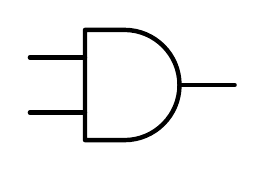
\begin{tikzpicture}[line width=1.6pt, line cap=round, line join=round]
        % Ingressi (linee orizzontali a sinistra)
        \draw (-0.7, 0.35) -- (0, 0.35);
        \draw (-0.7, -0.35) -- (0, -0.35);

        % Corpo della porta AND: lato posteriore dritto, tratti superiore/inferiore e arco semicircolare
        \draw (0, -0.7) -- (0, 0.7) -- (0.5, 0.7) arc[start angle=90, end angle=-90, radius=0.7] -- (0, -0.7);

        % Uscita (linea orizzontale a destra)
        \draw (1.2, 0) -- (1.9, 0);
    \end{tikzpicture}
\end{minipage}
\hfil
\begin{minipage}[c]{0.45\textwidth}
    \begin{tabular}{|c|c|c|}
        \hline
        $\mathbf{A}$ & $\mathbf{B}$ & $\mathbf{A \cdot B}$ \\ \hline
        0   &   0   &   0 \\ \hline
        0   &   1   &   0 \\ \hline
        1   &   0   &   0 \\ \hline
        1   &   1   &   1 \\ \hline
    \end{tabular}
\end{minipage}

\subsection{Porte OR}
\begin{minipage}{0.45\textwidth}
        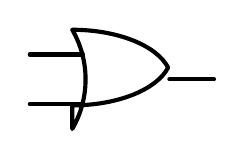
\begin{tikzpicture}[scale=0.9, line width=1.5pt, line cap=round, line join=round]
        % Ingressi (fermati esattamente sul bordo dell'arco)
        \draw (-0.7, 0.35) -- (0.05, 0.35);
        \draw (-0.7, -0.35) -- (0.05, -0.35);
    
        % Corpo della porta OR
        \draw (-0.1, -0.7) 
            arc[start angle=-30, end angle=30, radius=1.4] 
            arc[start angle=90, end angle=15, x radius=1.4, y radius=0.72]
            arc[start angle=-15, end angle=-90, x radius=1.4, y radius=0.72] 
            -- cycle;
    
        % Uscita (attaccata esattamente alla punta)
        \draw (1.27, 0) -- (1.9, 0);
    \end{tikzpicture}
\end{minipage}
\hfil
\begin{minipage}{0.45\textwidth}
    \begin{tabular}{|c|c|c|}
        \hline
        $\mathbf{A}$ & $\mathbf{B}$ & $\mathbf{A+B}$ \\ \hline
        0 & 0 & 0 \\ \hline
        0 & 0 & 0 \\ \hline
        0 & 0 & 0 \\ \hline
        0 & 0 & 0 \\\hline
    \end{tabular}
\end{minipage}


\subsection{Inverter}
\begin{minipage}{0.45\textwidth}
    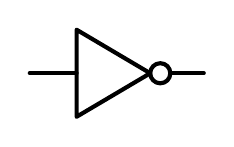
\begin{tikzpicture}[scale=0.85, line width=1.5pt, line cap=round, line join=round]
        % Ingresso
        \draw (-0.7, 0) -- (0, 0);
        % Triangolo
        \draw (0, -0.65) -- (0, 0.65) -- (1.1, 0) -- cycle;
        % Pallino di negazione
        \draw (1.25, 0) circle (0.15);
        % Uscita
        \draw (1.4, 0) -- (1.9, 0);
    \end{tikzpicture}
\end{minipage}
\hfil
\begin{minipage}{0.45\textwidth}
    \begin{tabular}{|c|c|}
        \hline
        $\mathbf{A}$ & $\mathbf{\overline{A}}$ \\ \hline
        0 & 1 \\ \hline
        1 & 0 \\ \hline
    \end{tabular}
\end{minipage}

\subsection{Multiplexer}
\begin{minipage}{0.45\textwidth}
    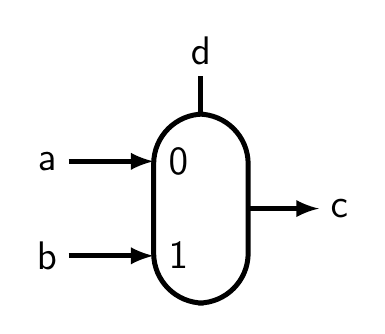
\begin{tikzpicture}[
            font=\sffamily\Large,
            thick,
            >=latex,
            scale=0.6
        ]

            % --- Corpo del Multiplexer (forma ovale allungata) ---
            \draw[line width=1.8pt, rounded corners=18pt] (0, 0) rectangle (2.0, 4);
            
            % Testi interni (0 e 1)
            \node[anchor=west] at (0.1, 3) {0};
            \node[anchor=west] at (0.1, 1) {1};

            % --- Ingressi a sinistra (a, b) ---
            \draw[->, line width=1.8pt] (-1.8, 3) node[left] {a} -- (0, 3);
            \draw[->, line width=1.8pt] (-1.8, 1) node[left] {b} -- (0, 1);

            % --- Segnale di selezione dall'alto (d) ---
            % Nota: L'immagine originale non ha la punta della freccia per l'ingresso 'd', 
            % ma solo una linea di connessione diretta.
            \draw[line width=1.8pt] (1.0, 4.8) node[above] {d} -- (1.0, 4);

            % --- Uscita a destra (c) ---
            \draw[->, line width=1.8pt] (2.0, 2) -- (3.5, 2) node[right] {c};

    \end{tikzpicture}
\end{minipage}
\hfil
\begin{minipage}{0.45\textwidth}
    \begin{tabular}{|c|c|}
        \hline \textbf{d} & \textbf{c} \\ \hline
        $0$ & a \\ \hline
        $1$ & b \\ \hline
    \end{tabular}
\end{minipage}

\section{ALU a 1 bit}
\subsection{Schema dettagliato ALU 30-0}
\begin{center}
    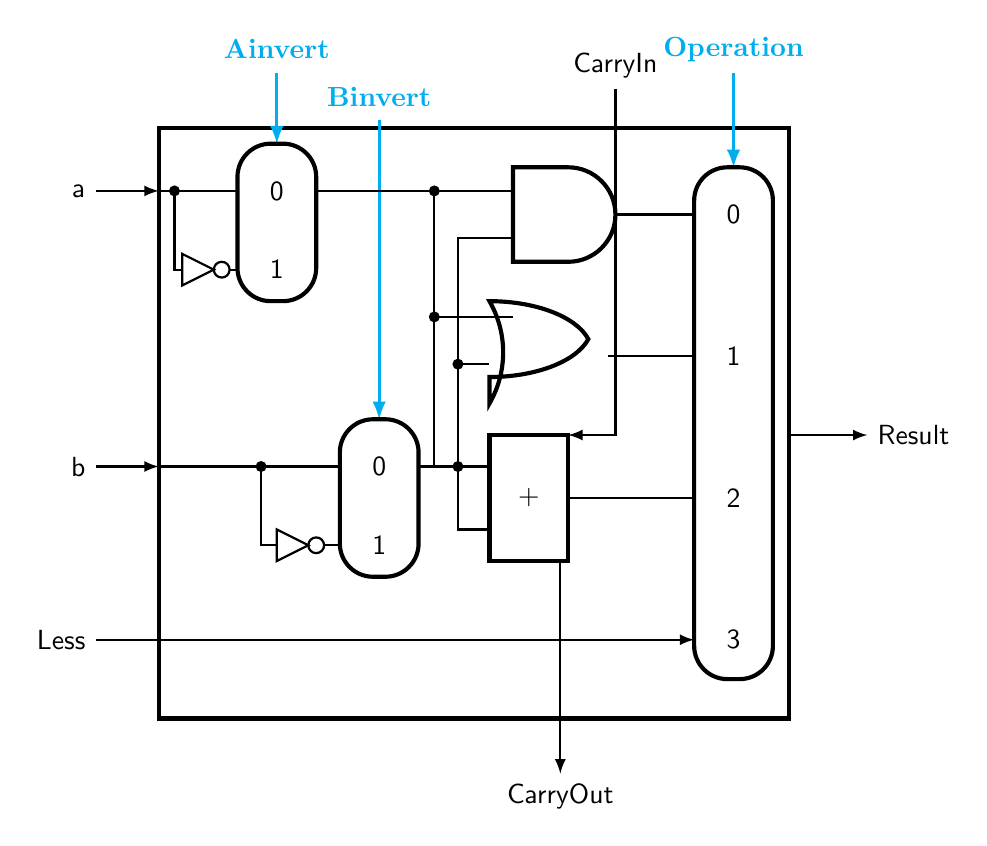
\begin{tikzpicture}[font=\sffamily, thick, >=latex]

        % --- Corpo Esterno del Blocco ALU ---
        \draw[line width=1.5pt] (0, -2.5) rectangle (8.0, 5.0);

        % --- 1. Ingressi e Frecce Principali (Lato Sinistro / Basso) ---
        \draw[->] (-0.8, 4.2) node[left] {a} -- (0, 4.2);
        \draw[->] (-0.8, 0.7) node[left] {b} -- (0, 0.7);
        \draw[->] (-0.8, -1.5) node[left] {Less} -- (6.8, -1.5);

        % --- 2. Ingressi di Controllo in Azzurro (Dall'alto) ---
        % Ainvert
        \node[text=cyan, font=\bfseries] at (1.5, 6.0) {Ainvert};
        \draw[->, color=cyan, line width=1.2pt] (1.5, 5.7) -- (1.5, 4.8);

        % Binvert
        \node[text=cyan, font=\bfseries] at (2.8, 5.4) {Binvert};
        \draw[->, color=cyan, line width=1.2pt] (2.8, 5.1) -- (2.8, 1.3);

        % Operation
        \node[text=cyan, font=\bfseries] at (7.3, 6.0) {Operation};
        \draw[->, color=cyan, line width=1.2pt] (7.3, 5.7) -- (7.3, 4.5);

        % CarryIn
        \draw (5.8, 5.5) node[above] {CarryIn} -- (5.8, 5.0);
        \draw[->] (5.8, 5.0) -- (5.8, 1.1) -- (5.2, 1.1); % Scende verso il Sommatore
        
        % --- 3. Uscite (Destra / Basso) ---
        \draw[->] (8.0, 1.1) -- (9.0, 1.1) node[right] {Result};
        \draw[->] (5.1, -0.5) -- (5.1, -3.2) node[below] {CarryOut};

        % ==========================================
        % 4. COMPONENTI INTERNI
        % ==========================================
        
        % --- MUX A (Ainvert) ---
        \draw[line width=1.5pt, rounded corners=12pt] (1.0, 2.8) rectangle (2.0, 4.8);
        \node at (1.5, 4.2) {0};
        \node at (1.5, 3.2) {1};
        
        \fill (0.2, 4.2) circle (0.07);
        \draw (0, 4.2) -- (1.0, 4.2); % Linea a diretta
        
        % Linea a negata (Porta NOT)
        \draw (0.2, 4.2) -- (0.2, 3.2) -- (0.3, 3.2);
        \draw (0.3, 3.0) -- (0.3, 3.4) -- (0.7, 3.2) -- cycle; % Triangolo NOT
        \draw (0.8, 3.2) circle (0.1); % Pallino
        \draw (0.9, 3.2) -- (1.0, 3.2);

        % --- MUX B (Binvert) ---
        \draw[line width=1.5pt, rounded corners=12pt] (2.3, -0.7) rectangle (3.3, 1.3);
        \node at (2.8, 0.7) {0};
        \node at (2.8, -0.3) {1};
        
        \fill (1.3, 0.7) circle (0.07);
        \draw (0, 0.7) -- (2.3, 0.7); % Linea b diretta

        % Linea b negata (Porta NOT)
        \draw (1.3, 0.7) -- (1.3, -0.3) -- (1.5, -0.3);
        \draw (1.5, -0.5) -- (1.5, -0.1) -- (1.9, -0.3) -- cycle; % Triangolo NOT
        \draw (2.0, -0.3) circle (0.1); % Pallino
        \draw (2.1, -0.3) -- (2.3, -0.3);


        % --- Porta AND ---
        \draw[line width=1.5pt] (4.5, 3.3) -- (4.5, 4.5) -- (5.2, 4.5) arc[start angle=90, end angle=-90, radius=0.6] -- cycle;
        
        % --- Porta OR ---
        \draw[line width=1.5pt] (4.2, 1.5) 
            arc[start angle=-30, end angle=30, radius=1.3] 
            arc[start angle=90, end angle=15, x radius=1.3, y radius=0.65]
            arc[start angle=-15, end angle=-90, x radius=1.3, y radius=0.65] 
            -- cycle;

        % --- Sommatore (Adder) ---
        \draw[line width=1.5pt] (4.2, -0.5) rectangle (5.2, 1.1);
        \node at (4.7, 0.3) {$+$};


        % ==========================================
        % 5. COLLEGAMENTI TRA I COMPONENTI
        % ==========================================

        % --- Da MUX A verso le porte (AND, OR, +) ---
        \draw (2.0, 4.2) -- (3.5, 4.2);
        \fill (3.5, 4.2) circle (0.07);
        
        \draw (3.5, 4.2) -- (4.5, 4.2); % Verso AND
        
        \draw (3.5, 4.2) -- (3.5, 2.6);
        \fill (3.5, 2.6) circle (0.07);
        \draw (3.5, 2.6) -- (4.5, 2.6); % Verso OR
        
        \draw (3.5, 2.6) -- (3.5, 0.7); 
        \draw (3.5, 0.7) -- (4.2, 0.7); % Verso Adder

        % --- Da MUX B verso le porte (AND, OR, +) ---
        \draw (3.3, 0.7) -- (3.8, 0.7);
        \fill (3.8, 0.7) circle (0.07);
        
        \draw (3.8, 0.7) -- (3.8, 3.6) -- (4.5, 3.6); % Verso AND
        
        \fill (3.8, 2.0) circle (0.07);
        \draw (3.8, 2.0) -- (4.2, 2.0); % Verso OR
        
        \draw (3.8, 0.7) -- (3.8, -0.1) -- (4.2, -0.1); % Verso Adder


        % --- MUX Finale (Operation) ---
        \draw[line width=1.5pt, rounded corners=12pt] (6.8, -2.0) rectangle (7.8, 4.5);
        \node at (7.3, 3.9) {0};
        \node at (7.3, 2.1) {1};
        \node at (7.3, 0.3) {2};
        \node at (7.3, -1.5) {3};
        
        % --- Collegamenti finali a MUX Operation ---
        \draw (5.8, 3.9) -- (6.8, 3.9); % Da AND (0)
        \draw (5.7, 2.1) -- (6.8, 2.1); % Da OR (1)
        \draw (5.2, 0.3) -- (6.8, 0.3); % Da Adder (2)
        % (3) L'ingresso Less arriva direttamente dalla sinistra (già disegnato sopra)

    \end{tikzpicture}
\end{center}

\subsection{Schema dettagliato ALU 31}
\begin{center}
    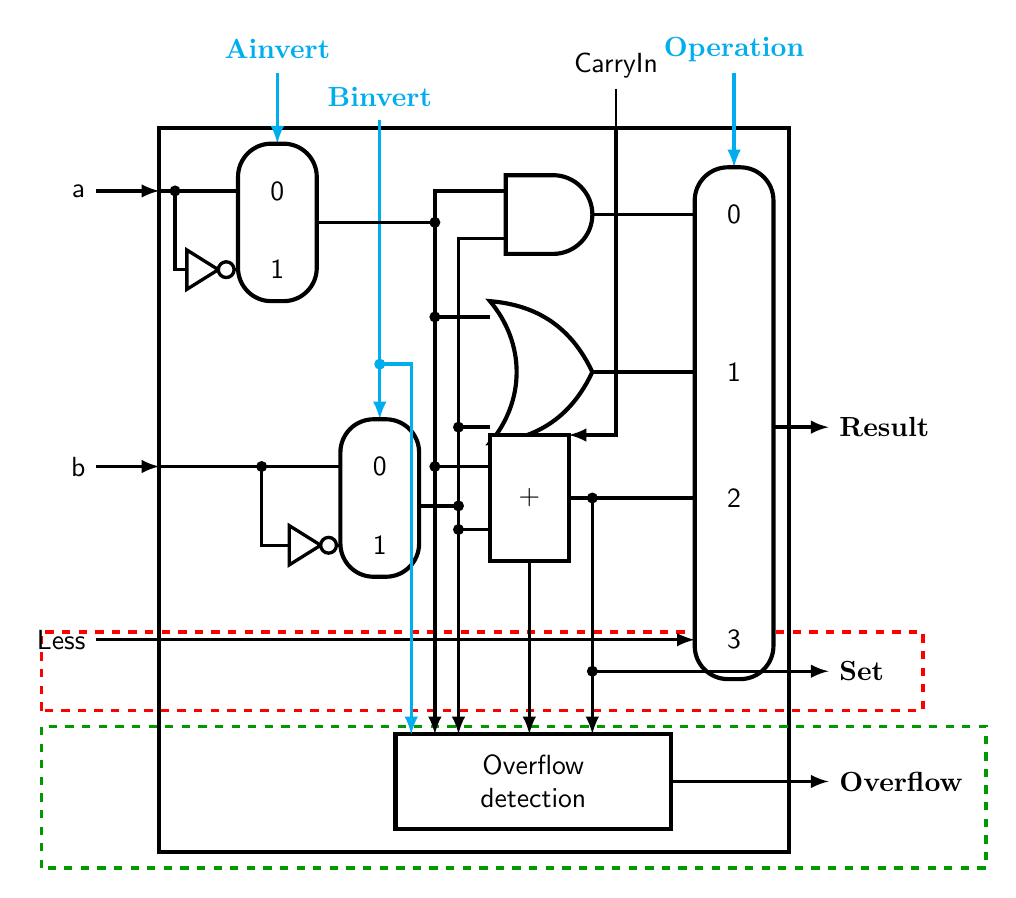
\begin{tikzpicture}[font=\sffamily, thick, >=latex]

        % ==========================================
        % 1. PERIMETRI E RIQUADRI TRATTEGGIATI
        % ==========================================
        
        % Riquadro principale dell'ALU (Nero)
        \draw[line width=1.5pt] (0, -4.2) rectangle (8.0, 5.0);

        % Riquadro tratteggiato Rosso (attorno a Set)
        \draw[dashed, red, line width=1.2pt] (-1.5, -2.4) rectangle (9.7, -1.4);

        % Riquadro tratteggiato Verde (attorno a Overflow)
        \draw[dashed, green!60!black, line width=1.2pt] (-1.5, -4.4) rectangle (10.5, -2.6);


        % ==========================================
        % 2. INGRESSI PRINCIPALI (Sinistra e Alto)
        % ==========================================
        
        % Ingressi a, b, Less
        \draw[->, line width=1.2pt] (-0.8, 4.2) node[left] {a} -- (0, 4.2);
        \draw[->, line width=1.2pt] (-0.8, 0.7) node[left] {b} -- (0, 0.7);
        \draw[->, line width=1.2pt] (-0.8, -1.5) node[left] {Less} -- (6.8, -1.5);

        % Segnali di controllo (Azzurro)
        \node[text=cyan, font=\bfseries] at (1.5, 6.0) {Ainvert};
        \draw[->, color=cyan, line width=1.2pt] (1.5, 5.7) -- (1.5, 4.8);

        \node[text=cyan, font=\bfseries] at (2.8, 5.4) {Binvert};
        \draw[->, color=cyan, line width=1.2pt] (2.8, 5.1) -- (2.8, 1.3);

        \node[text=cyan, font=\bfseries] at (7.3, 6.0) {Operation};
        \draw[->, color=cyan, line width=1.2pt] (7.3, 5.7) -- (7.3, 4.5);

        % CarryIn (Nero)
        \draw (5.8, 5.5) node[above] {CarryIn} -- (5.8, 5.0);
        \draw[->, line width=1.2pt] (5.8, 5.0) -- (5.8, 1.1) -- (5.2, 1.1);


        % ==========================================
        % 3. MULTIPLEXER A e B (con porte NOT)
        % ==========================================
        
        % --- MUX A ---
        \draw[fill=white, line width=1.5pt, rounded corners=12pt] (1.0, 2.8) rectangle (2.0, 4.8);
        \node at (1.5, 4.2) {0}; \node at (1.5, 3.2) {1};
        
        \fill (0.2, 4.2) circle (0.07);
        \draw[line width=1.2pt] (0, 4.2) -- (1.0, 4.2);
        
        \draw[line width=1.2pt] (0.2, 4.2) -- (0.2, 3.2) -- (0.35, 3.2);
        \draw[fill=white, line width=1.2pt] (0.35, 2.95) -- (0.35, 3.45) -- (0.75, 3.2) -- cycle; % NOT
        \draw[fill=white, line width=1.2pt] (0.85, 3.2) circle (0.1);
        \draw[line width=1.2pt] (0.95, 3.2) -- (1.0, 3.2);

        % --- MUX B ---
        \draw[fill=white, line width=1.5pt, rounded corners=12pt] (2.3, -0.7) rectangle (3.3, 1.3);
        \node at (2.8, 0.7) {0}; \node at (2.8, -0.3) {1};
        
        \fill (1.3, 0.7) circle (0.07);
        \draw[line width=1.2pt] (0, 0.7) -- (2.3, 0.7);
        
        \draw[line width=1.2pt] (1.3, 0.7) -- (1.3, -0.3) -- (1.65, -0.3);
        \draw[fill=white, line width=1.2pt] (1.65, -0.55) -- (1.65, -0.05) -- (2.05, -0.3) -- cycle; % NOT
        \draw[fill=white, line width=1.2pt] (2.15, -0.3) circle (0.1);
        \draw[line width=1.2pt] (2.25, -0.3) -- (2.3, -0.3);


        % ==========================================
        % 4. COMPONENTI CENTRALI (AND, OR, ADDER, OVERFLOW)
        % ==========================================
        
        % Porta AND
        \draw[fill=white, line width=1.5pt] (4.4, 3.4) -- (4.4, 4.4) -- (5.0, 4.4) arc(90:-90:0.5) -- cycle;
        
        % Porta OR
        \draw[fill=white, line width=1.5pt] (4.2, 1.0) to[bend right=40] (4.2, 2.8) to[bend left=30] (5.5, 1.9) to[bend left=30] cycle;

        % Sommatore (Adder)
        \draw[fill=white, line width=1.5pt] (4.2, -0.5) rectangle (5.2, 1.1);
        \node at (4.7, 0.3) {$+$};

        % Blocco Overflow detection
        \draw[fill=white, line width=1.5pt] (3.0, -3.9) rectangle (6.5, -2.7);
        \node[align=center] at (4.75, -3.3) {Overflow\\detection};


        % ==========================================
        % 5. COLLEGAMENTI INTERNI (ROUTING)
        % ==========================================
        
        % --- Derivazione Binvert verso Overflow (Azzurro) ---
        \fill[cyan] (2.8, 2.0) circle (0.07);
        \draw[->, cyan, line width=1.2pt] (2.8, 2.0) -- (3.2, 2.0) -- (3.2, -2.7);

        % --- Linea da MUX A ---
        \draw[line width=1.2pt] (2.0, 3.8) -- (3.5, 3.8);
        \fill (3.5, 3.8) circle (0.07);
        \draw[line width=1.2pt] (3.5, 3.8) -- (3.5, 4.2) -- (4.4, 4.2); % Verso AND
        \draw[line width=1.2pt] (3.5, 3.8) -- (3.5, 2.6) -- (4.2, 2.6); % Verso OR
        \fill (3.5, 2.6) circle (0.07);
        \draw[line width=1.2pt] (3.5, 2.6) -- (3.5, 0.7) -- (4.2, 0.7); % Verso Adder
        \fill (3.5, 0.7) circle (0.07);
        \draw[->, line width=1.2pt] (3.5, 0.7) -- (3.5, -2.7); % Verso Overflow detection

        % --- Linea da MUX B ---
        \draw[line width=1.2pt] (3.3, 0.2) -- (3.8, 0.2);
        \fill (3.8, 0.2) circle (0.07);
        \draw[line width=1.2pt] (3.8, 0.2) -- (3.8, 3.6) -- (4.4, 3.6); % Verso AND
        \draw[line width=1.2pt] (3.8, 0.2) -- (3.8, 1.2) -- (4.2, 1.2); % Verso OR
        \fill (3.8, 1.2) circle (0.07);
        \draw[line width=1.2pt] (3.8, 0.2) -- (3.8, -0.1) -- (4.2, -0.1); % Verso Adder
        \fill (3.8, -0.1) circle (0.07);
        \draw[->, line width=1.2pt] (3.8, -0.1) -- (3.8, -2.7); % Verso Overflow detection

        % --- Linea CarryOut dall'Adder ---
        \draw[->, line width=1.2pt] (4.7, -0.5) -- (4.7, -2.7); % Verso Overflow detection


        % ==========================================
        % 6. MULTIPLEXER OPERATION E USCITE
        % ==========================================
        
        % --- MUX Finale (Operation) ---
        \draw[fill=white, line width=1.5pt, rounded corners=12pt] (6.8, -2.0) rectangle (7.8, 4.5);
        \node at (7.3, 3.9) {0};
        \node at (7.3, 1.9) {1};
        \node at (7.3, 0.3) {2};
        \node at (7.3, -1.5) {3};
        
        % Ingressi al MUX
        \draw[line width=1.2pt] (5.5, 3.9) -- (6.8, 3.9); % Da AND
        \draw[line width=1.2pt] (5.5, 1.9) -- (6.8, 1.9); % Da OR
        
        % Output Adder -> MUX e diramazioni (Set e Overflow)
        \draw[line width=1.2pt] (5.2, 0.3) -- (6.8, 0.3); % Verso MUX
        \fill (5.5, 0.3) circle (0.07);
        \draw[->, line width=1.2pt] (5.5, 0.3) -- (5.5, -2.7); % Continua dritto verso Overflow
        
        \fill (5.5, -1.9) circle (0.07);
        \draw[->, line width=1.2pt] (5.5, -1.9) -- (8.5, -1.9) node[right, font=\bfseries] {Set}; % Uscita Set

        % --- Uscita Result ---
        \draw[->, line width=1.2pt] (7.8, 1.2) -- (8.5, 1.2) node[right, font=\bfseries] {Result};

        % --- Uscita Overflow ---
        \draw[->, line width=1.2pt] (6.5, -3.3) -- (8.5, -3.3) node[right, font=\bfseries] {Overflow};

    \end{tikzpicture}
\end{center}

\newpage
\subsection{Operazioni disponibili}
\begin{itemize}
    \item Addizione (con CarryIn e CarryOut)
    \item Sottrazione ($a-b = a + \text{CA2(b)}$)
    \item SLT
    \item Overflow detection
\end{itemize}

\subsection{Operazione SLT - Set on Less Then}
\subsubsection{Cosa fa?}
Poni registro1 = 1 se il valore contenuto in registro 2 è minore del valore contenuto in registro 3
\begin{itemize}
    \item 1 se $a<b$, $0$ altrimenti
\end{itemize}

\subsubsection{Come funziona?}
Per eseguire questa istruzione si devono poter azzerare tutti i bit dal bit-1 al bit-31 ed assegnare al bit-0 il valore risultato dell'operazione di slt.

\begin{minipage}{0.45\textwidth}
{
    \Large
    $$
        a<b
    $$
}
\end{minipage}
\hfil
\begin{minipage}{0.45\textwidth}
    \begin{enumerate}
        \item $a-b<0$
        \item La sottrazione $(a-b)$ è negativa
        \item Bit-31 della sottrazione $(a-b)=1$
    \end{enumerate}
\end{minipage}

\vspace{0.2cm}

Per poter realizzare il confronto si effettua la sottrazione tra a e b
\begin{itemize}
    \item Se $a-b$ è minore di $0$, allora $a<b$ (per l'istruzione slt)
    \begin{itemize}
        \item Il risultato sarà $00\dots01$
    \end{itemize}
    \item Se $a-b$ è maggiore di $0$, allora $a>b$ (per l'istruzione slt)
    \begin{itemize}
        \item Il risultato sarà $00\dots00$
    \end{itemize}
\end{itemize}

\subsection{Overflow detection}
\subsubsection{Cosa fa?}
Controlla se un operazione sfora il numero di bit a disposizione

\subsection{Casi di Overflow}
\begin{itemize}
    \item $(A-B)>0$ e bit-31 di $(A-B)=1$ oppure
    \item $(A-B)>0$ e bit-31 di $(A-B)=0$
\end{itemize}

\vspace{0.3cm}

\begin{center}
    \begin{tcolorbox}[width=0.65\textwidth]
        \begin{center}
            $\text{bit-31(A)}=0, \ \text{bit-31(B)}=1 \to  \text{bit-31(A-B)}=1$
            
            \vspace{0.3cm}

            oppure

            \vspace{0.3cm}

            $\text{bit-31(A)}=1,\ \text{bit-31(B)=0} \to \text{bit-31(A-B)}=0$
        \end{center}
    \end{tcolorbox}
\end{center}

\vspace{0.3cm}

\subsubsection{Come funziona}
{
    \Large
    $$
    \text{overflow} = \overline{a} \cdot b \cdot \text{Result} + a \cdot \overline{b} \cdot \overline{\text{Result}}
    $$
}


\section{ALU a 32 bit}

\subsection{Schema dettagliato}
\begin{center}
    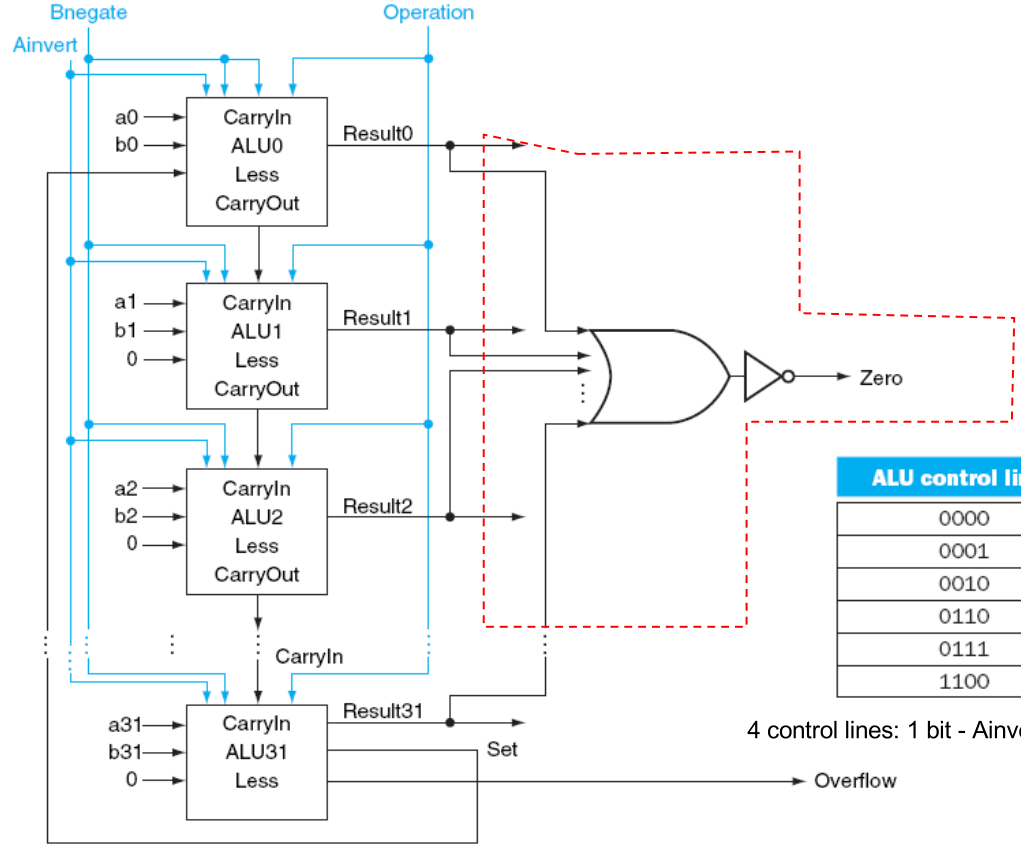
\includegraphics[scale=0.5]{Immagini/ALU-32Bit.png}
\end{center}

\begin{minipage}[t]{0.45\textwidth}
\subsection{Schema semplificato}
    \begin{center}
    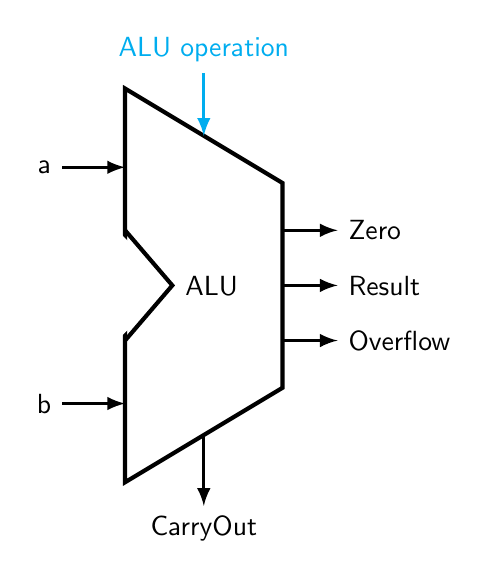
\begin{tikzpicture}[font=\sffamily, thick, >=latex]
    
        % --- Corpo dell'ALU ---
        % Disegna il perimetro principale con l'intaglio a sinistra (forma a V)
        \draw[line width=1.5pt] (0, 0) -- (0, 5) -- (2, 3.8) -- (2, 1.2) -- cycle;
        
        % Intaglio centrale (V rovesciata sul dorso sinistro)
        \draw[fill=white, draw=none] (-0.1, 1.8) -- (0.6, 2.5) -- (-0.1, 3.2) -- cycle; % mask
        \draw[line width=1.5pt] (0, 3.2) -- (0.6, 2.5) -- (0, 1.8);
        
        \node at (1.1, 2.5) {ALU};
    
        % --- Ingressi a sinistra (a, b) ---
        \draw[->, line width=1.2pt] (-0.8, 4.0) node[left] {a} -- (0, 4.0);
        \draw[->, line width=1.2pt] (-0.8, 1.0) node[left] {b} -- (0, 1.0);
    
        % --- Ingresso dall'alto (ALU operation) in azzurro ---
        \node[text=cyan] at (1.0, 5.5) {ALU operation};
        \draw[->, cyan, line width=1.2pt] (1.0, 5.2) -- (1.0, 4.4);
    
        % --- Uscite a destra ---
        \draw[->, line width=1.2pt] (2.0, 3.2) -- (2.7, 3.2) node[right] {Zero};
        \draw[->, line width=1.2pt] (2.0, 2.5) -- (2.7, 2.5) node[right] {Result};
        \draw[->, line width=1.2pt] (2.0, 1.8) -- (2.7, 1.8) node[right] {Overflow};
    
        % --- Uscita in basso (CarryOut) ---
        \draw[->, line width=1.2pt] (1.0, 0.6) -- (1.0, -0.3) node[below] {CarryOut};
    
    \end{tikzpicture}
    \end{center}
\end{minipage}
\hfil
\begin{minipage}[t]{0.45\textwidth}
\subsection{Tabella di controllo}
    \begin{center}
    \begin{tabular}{|c|c|}
        \hline \textbf{Codice} & \textbf{Funzione} \\ \hline
        \texttt{0000} & AND \\ \hline
        \texttt{0001} & OR \\ \hline
        \texttt{0010} & ADD \\ \hline
        \texttt{0110} & SUB \\ \hline
        \texttt{0111} & SLT \\ \hline
        \texttt{1100} & NOR \\ \hline
    \end{tabular}
\end{center}
\end{minipage}

\subsection{Operazione BEQ - Branch on equal}

\subsubsection{Cosa fa?}

\vspace{0.5cm}

\begin{center}
    {
        \large
        \texttt{beq registro1, registro2, L1}
    }
\end{center}

\vspace{0.5cm}

L'istruzione ti fa saltare all'etichetta L1 se il valore contenuto in registro1 è uguale al valore contenuto in registro 2

\subsubsection{Come funziona?}
Per verificare l'uguaglianza di a e b si effettua una sottrazione

Se $a=b$ allora dobbiamo mettere a 1 la linea di output usata per l'uguagliaanza, oppure si fa l'OR di tutte le uscite e poi si nega il risultato